\documentclass[a4paper,10pt]{article}
\usepackage[utf8]{inputenc}
\usepackage{glossaries}
\usepackage{fullpage}
\usepackage{hyperref}
\usepackage{amsmath}
\usepackage{graphicx}
\usepackage{subcaption}
\usepackage{verbatim}
\usepackage{pgfplots, pgfplotstable}
\setlength\parindent{0pt}
\setlength{\parskip}{10pt}

\makeglossaries
\newglossaryentry{vlbi}{%
name={VLBI},%
description={Very Long Baseline Interferometry}%
}
\newglossaryentry{fir}{%
name={FIR},%
description={Finite Impulse Response}%
}
\newglossaryentry{pfb}{%
name={PFB},%
description={Polyphase Filter Bank}%
}
\newglossaryentry{lo}{%
name={lo},%
description={Local Oscillator}%
}
\newglossaryentry{pr}{%
name={PR},%
description={Perfect Reconstruction}%
}
\newglossaryentry{fpga}{%
name={FPGA},%
description={Field Programmable Gate Array}%
}
\newglossaryentry{dft}{%
name={DFT},%
description={Discrete Fourier Transform}%
}
\newglossaryentry{fft}{%
name={FFT},%
description={Fast Fourier Tranform is a fast algorithm for computing the \gls{dft} using the Cooley–Tukey algorithm amongst others}%
}

\begin{document}
\begin{titlepage}

\newcommand{\HRule}{\rule{\linewidth}{0.5mm}} % Defines a new command for the horizontal lines, change thickness here

\center % Center everything on the page
 
%----------------------------------------------------------------------------------------
%	HEADING SECTIONS
%----------------------------------------------------------------------------------------

\textsc{\LARGE Square Kilometer Array South Africa}\\[1.5cm]
\textsc{\Large Internship technical report}\\[0.5cm]

%----------------------------------------------------------------------------------------
%	TITLE SECTION
%----------------------------------------------------------------------------------------

\HRule \\[0.4cm]
{ \huge \bfseries KAT-7 GPU-accelerated Inverse Polyphase Filterbank}\\[0.4cm]
\HRule \\[1.5cm]
 
%----------------------------------------------------------------------------------------
%	AUTHOR SECTION
%----------------------------------------------------------------------------------------

\begin{minipage}{0.4\textwidth}
\begin{flushleft} \large
\emph{Author:}\\
Benjamin \textsc{Hugo}\\[0.2cm] % Your name
\small{Department of Computer Science}\\
\small{University of Cape Town}\\
\small{bennahugo@aol.com}

\end{flushleft}
\end{minipage}
~
\begin{minipage}{0.4\textwidth}
\begin{flushright} \large
\emph{Advisor:} \\
Ludwig Schwardt
\end{flushright}
\end{minipage}\\[4cm]

% If you don't want a supervisor, uncomment the two lines below and remove the section above
%\Large \emph{Author:}\\
%John \textsc{Smith}\\[3cm] % Your name

%----------------------------------------------------------------------------------------
%	DATE SECTION
%----------------------------------------------------------------------------------------

{\large \today}\\[3cm] % Date, change the \today to a set date if you want to be precise
{The results obtained in this report was made possible through the use of the ICTS High Performance HEX cluster 
of the University of Cape Town (UCT) \url{hex.uct.ac.za}. The author wishes to thank Andrew Lewis of UCT ICTS for 
the technical support he provided during this project.}
%----------------------------------------------------------------------------------------
%	LOGO SECTION
%----------------------------------------------------------------------------------------

%\includegraphics{Logo}\\[1cm] % Include a department/university logo - this will require the graphicx package
 
%----------------------------------------------------------------------------------------

\vfill % Fill the rest of the page with whitespace

\end{titlepage}

\printglossary[style=long]
\pagebreak
\tableofcontents
\pagebreak
\section{Introduction}
At its core Very Long Baseline Interferometry (\gls{vlbi}) is an interferometry process where the output from several radio antennae are 
combined, to form an equivalent output to a telescope of the size equal to the distance between the furthest two antennae in the \gls{vlbi} array.
For a comprehensive overview of the technique the reader is referred to the detailed introduction by Middelberg et al. \cite{middelberg2008high}. Several
such extended arrays exist including the European VLBI network and the Very Long Baseline Array. The hope is to include the KAT-7 in future VLBI
observations.

Traditionally the process required raw data to be dumped to a storage medium, say tape and physically shipped to a correlator where the data from several 
telescopes could be combined. The new trend in VLBI is to perform real-time correlation between antennae using high-speed internet connections and is known
as 'eVLBI'. Both the Australian Long Baseline Array and the European VLBI network have performed successful eVLBI observations.

Ultimately the problem being investigated (at least in part by this report) can be boiled down to converting data sent over the SPEAD protocol (employed 
internally by the KAT-7 array) to the VDIF format. This conversion process includes a necessary first step, where the current sampling rate of 800 MHz
\footnote{According to the KAT-7 Data Interface document} is reduced to 128 MHz through \textit{Digital Downconversion}. The basic operation involves the following three
steps:
\begin{enumerate}
 \item Mixing. Where the signal is shifted down to \textit{baseband} (frequency 0 of the spectrum), by mixing the signal with a tone produced by a Local Oscillator (\gls{lo}).
 This is simply a generated sine wave at the lower end of the sub-spectrum to be extracted. This is simply done by an element-wise multiplication of the original signal with
 the local oscillator tone. In essence mixing is not a \textit{linear} (refer to \cite[ch. 5]{smith1997scientist}) process. If $f$ was a single channel in the 
 frequency domain then mixing produces replicated channels at $f - f_{lo}$ and $f + f_{lo}$.
 \item Filtering. In order to eliminate aliasing in the frequency domain due to mixing and frequencies above the new sampling rate we use a Finite Impulse Response 
 (\gls{fir}) filter with the cutoff set at the rate $\frac{1}{2}f_{decimated}$ to comply with the Nyquest sampling theorem (see \cite[ch. 3]{smith1997scientist}).
 \item Interpolation and Decimation. The reader is referred to \url{http://www.dspguru.com/dsp/faqs/multirate/basics} for an overview of the process.  
\end{enumerate}

There is, however, a further complication to deal with, before this downconversion process can begin. The KAT-7 beamformer produces a series of frequency spectra. If no filtering 
was applied to these spectra, the undo operation would only have involved applying the inverse Discrete Fourier Transform (\gls{dft}). However, the original voltage data went 
through a filter-bank operation, in a process known as the Polyphase Filter Bank (\gls{pfb}). This method is also known as the Weighted Window Overlap method and is necessary for computing 
Short Time Discrete Fourier Transforms subsections of very long signals. The reader is referred to \url{https://casper.berkeley.edu/wiki/The_Polyphase_Filter_Bank_Technique} for a detailed 
description on the forward \gls{pfb}.

\section{Method}
\subsection{Validation of the forward and inverse processes}
The forward \gls{pfb} process can be thought of as a very basic analysis filter bank, whereas the inverse process can be thought of as a synthesis filter bank. The 
analysis filter bank uses a Hamming-windowed \gls{fir} with $P=8$ banks of $N=1024$ elements, with no up or down-sampling stages \footnote{According to information provided by Jason Manley}.
Our implementation focusses on 8-bit sized samples produced by the KAT-7 beamformer \footnote{According to the KAT-7 Data Interface document}, but could easily adapted to other sample-sizes,
as well as prototype filter lengths.

The key differences between the analysis and synthesis processes are:
\begin{enumerate}
 \item If $H[n]$ is the prototype FIR filter and the analysis filter bank uses the subfilters $H_1[n], H_2[n] \dots H_P[n]$ each of length $N$ then the synthesis filter bank
 uses the subfilters $\bar H_1[N-n-1], \bar H_2[N-n-1] \dots \bar H_P[N-n-1]$\footnote{Findings published in an in-house final technical report titled 'A review of polyphase filter 
 banks and their application'. Daniel Zhou. Air Force Research Laboratory, Information Directorate, Rome Research Site, Rome, New York.}
 \item The commutator is flipped around (as shown on page 10 of Zhou's report) and therefore the sub filters should be processed in reverse order.
\end{enumerate}

We've implemented both the basic analysis and synthesis filter banks, as well as the necessary tools to analyse the performance of this basic filter bank construction. As shown in 
figure~\ref{filtered_and_unfiltered_analysis} the analysis filter bank successfully limits leakage of any frequencies that lie between neighbouring bin centers of the \gls{dft}.
This confirms that our basic analysis filter bank construction is correct.
\begin{figure}[h]
 \begin{subfigure}{0.5\textwidth}
  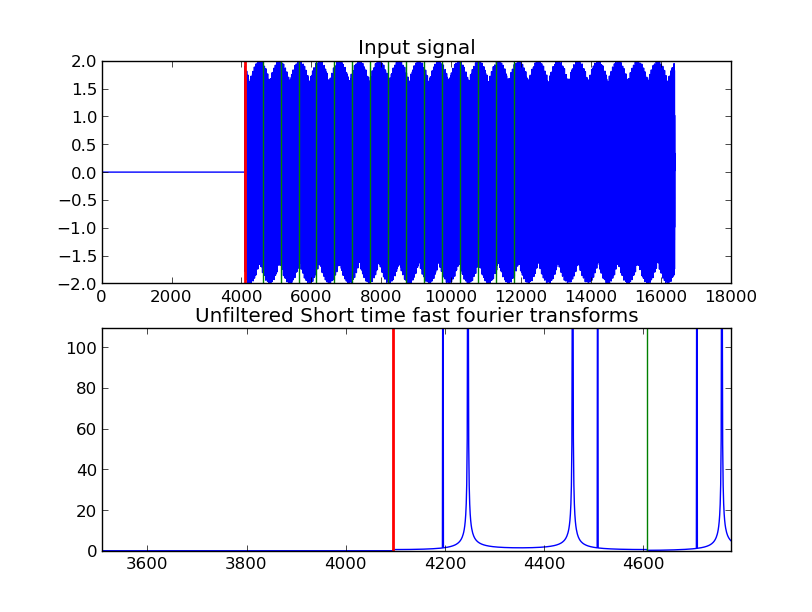
\includegraphics[width=0.95\textwidth]{unfiltered.png}
  \caption{Unfiltered analysis filter bank}
 \end{subfigure}
 \begin{subfigure}{0.5\textwidth}
  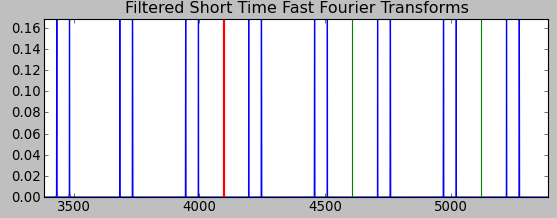
\includegraphics[width=0.95\textwidth]{filtered.png}
  \caption{Filtered analysis filter bank}
 \end{subfigure}
\caption{Example of \gls{dft} leakage. It is clear that the unfiltered analysis filter bank suffers severely when containing frequencies even slightly off the bin centers
	 of the \gls{dft}. Its filtered counterpart produces crisp binning of both centered and uncentered frequencies.}
\label{filtered_and_unfiltered_analysis}
\end{figure}

The synthesis filter bank construction was tested through cross correlation with the original input signal. A surefire way of determining if there is a 
correlation between the two intput and output of the sythesis filter bank, is to use Gaussian noise as input signal. Perfect Reconstruction (\gls{pr}) requires that the signal 
only varies in the following two ways:
\begin{enumerate}
 \item The output signal may be shifted by some $\Delta$ time steps.
 \item The output signal may be scaled by a constant.
\end{enumerate}

The signal shift may be found by the following method (where $x[t]$ is the input to the analysis filter and $y[t]$ is the output of the synthesis filter):
\begin{equation}
 \Delta=\underset{t}{argmax}(x[t]\star y[t])
\end{equation}

According to Parishwad Vaidyanathan \cite{vaidyanathan1990multirate} this basic filter bank cannot achieve \gls{pr} and have to be modified in order to do so. This involves 
modifying both the analysis and synthesis filter banks. In our situation this is not plausible, since the only the basic form of analysis filter bank is implemented 
on Field Programmable Gate Arrays (\gls{fpga}) due to their simple construction and \textit{fast evaluation times} \cite{vaidyanathan1990multirate}. Vaidyanathan goes on to state, 
however, that the synthesis filter bank requires subfilters of much greater length to obtain reasonably good reconstruction and is therefore computationally prohibiting. That 
said, as the reader can see from figure~\ref{correlation}, $x[t]\star y[t]$ shows that our basic synthesis filter bank achieves limited reconstruction.

\begin{figure}
 \begin{subfigure}{0.5\textwidth}
  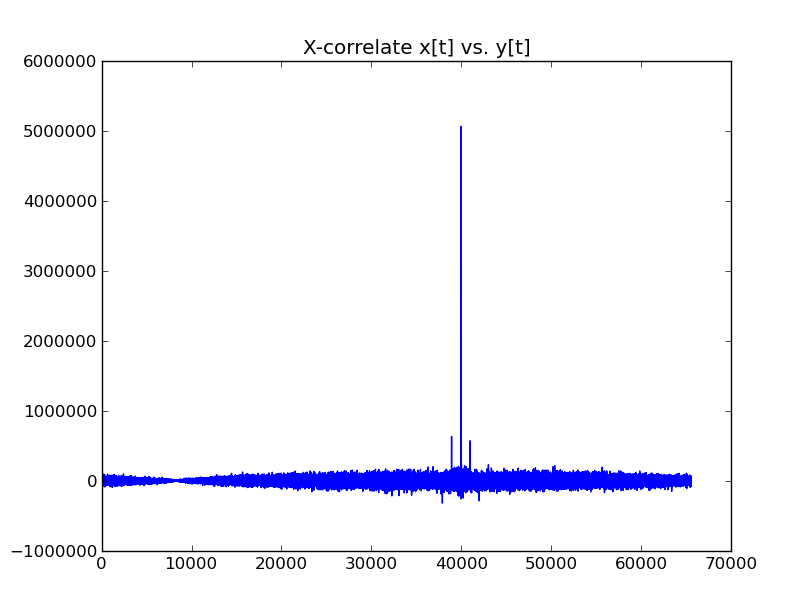
\includegraphics[width=0.95\textwidth]{x_cor.png}
  \caption{Cross correlation between $x[t]$ and $y[t]$}
 \end{subfigure}
 \begin{subfigure}{0.5\textwidth}
  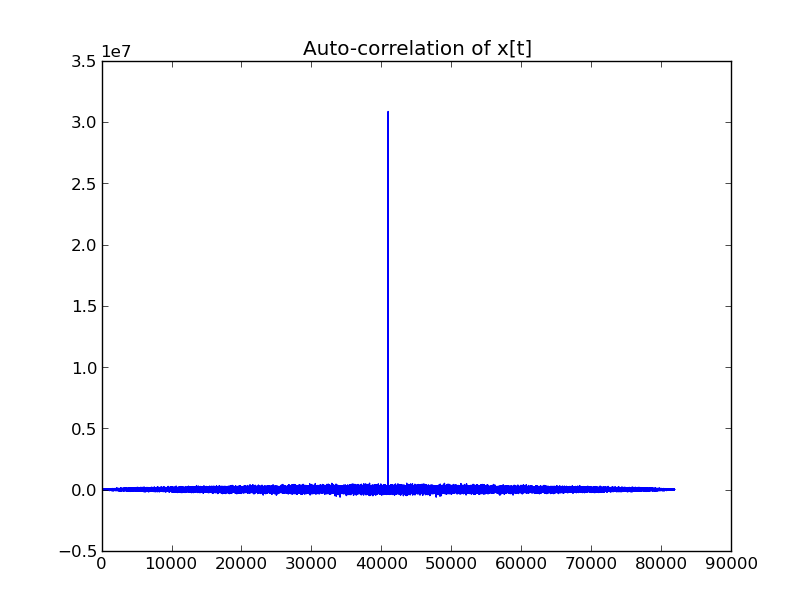
\includegraphics[width=0.95\textwidth]{auto_cor.png}
  \caption{Auto correlation of $x[t]$}
 \end{subfigure}
\caption{It is clear that even for Gaussian noise the synthesis filter bank achieves a limited reconstruction - the correlation between the reconstructed- and input signals is 
about 6 times weaker than the auto correlation of the input signal. The reader should also notice that it appears that $\Delta = -N\dot (P-1)$. This observation was made for 
trials with input signals of different lengths, but we have not rigorously proven this and it should not be taken as a fact. Future expansion, testing and debugging should use
the cross correlation to determine $\Delta$.}
\label{correlation}
\end{figure}

{\color{red} TODO:::::Discuss SNR once Ludwig has confirmed it is correct...}

\subsection{Validation of the GPU version}
We will for now only focus on the most basic construction to determine what throughput rates can be achieved, as well as the quality of the reconstruction. The full source code
along with test and analysis suite should be included with this report. With this suite the C++ CUDA GPU code is validated against a serial python implementation. The reader 
should have GCC 4.6 installed, along with the NVIDIA NVCC compiler toolkit 5.0 redistributable. Although the code should work on any platform, we have only tested this under 
recent GNU/Linux kernels. Another requirement is that the user have a Compute Capability $\geq2.0$ installed on their system. To run the test suite the user should have 
Python 2.7 along with the SciLab suite of packages installed (including NumPy, SciPy and MatPlotLab).

In order to validate that the GPU version is in fact producing valid results we've tested it against the output of our Python synthesis filter bank. The Mean Squared Error 
is defined as:
\begin{equation}
 MSE(input_1,input_2) := \frac{\sum_{k=0}^{L-1}{(input_1[k] - input_2[k])^2}}{L} \text{ where } ||input_1|| = ||input_2|| = L
\end{equation}

By generating 0.976 GiB of Gaussian noise we determined these following characteristics for the two output files:
\begin{center}
  \begin{tabular}{|c|c|c|}
    \hline
    \textbf{Metric} & \textbf{Python Synthesis Bank} & \textbf{GPU Synthesis Bank} \\
    \hline
    $\bar x$ & -0.000307 & -0.000307 \\
    \hline
    $\sigma^{2}$ & 2.969016 & 2.969015 \\
    \hline
    \textbf{Mean Squared Error} & \multicolumn{2}{|c|}{\textbf{0.000001}} \\
    \hline
  \end{tabular}
\end{center}

This subtle difference between the output files may be attributed to both floating-point rounding errors and the fact that we discarded the last non-redundant
sample of \gls{fft} output. Different \gls{fft} implementations may behave differently under this situation and may produce slightly different results. It should be noted
that here the GPU has processed the file in several batches as we will explain next.

\subsection{Optimizations on the GPU-accelerated synthesis filter bank}
The GPU version has been constructed with the requirements of real-time operation in mind. Although it has not been integrated into a SPEAD receiver, the device simply has
to be initialized once. The GPU will allocate all the memory it requires during this initialization process. After this initialization step the user can send batches of any size 
off to the GPU for processing on a rolling bases, as long as one batch is fully processed before the next batch is started. The GPU inverts all the \gls{dft}s in a combined operation  
and keeps track of the last $P\times N$ $N$-sized inverse \gls{dft}, by keeping a persistent buffer between batches. The only hard constraint placed on this batching process is that 
the size of the batch is an integral multiple of $N$ (the length of each analysis spectrum as mentioned earlier). At this point we wish to make the reader aware of subtlety in the 
output data received from the beamformers. Although a real-valued inverse \gls{dft} will require $\frac{N}{2}+1$ non-redundant samples to perform a computation the last frequency bin 
is discarded before we receive it. The author has assumed $X_{filtered}[f=\frac{N}{2}+1] = 0$ in his construction of the analysis and synthesis filterbanks.

Care has been taken in optimizing the GPU code according to the architectural requirements of GPUs: 
\begin{enumerate}
 \item Memory copies to and from the device is done in batches to improve latency
 \item Memory accesses have been coalesced, including necessary padding to align memory to the 128 byte memory boundaries of Compute Capability 2.0. This constant 
 can be adjusted for later architectures if necessary. At this point we should warn the reader that $N$ must be a multiple of 128 for this coalescing scheme to function
 as intended.
 \item Memory transfers to and from the GPU have been optimized by pinning host memory to primary memory so that they do not get paged out to disk by the memory 
 controller of the host operating system.
 \item DFTs are computed in batches using the NVIDIA cufft libraries using the Fast Fourier Transform.
 \item CUDA streams are used to run kernels and memory copies asynchronously whenever possible. This adds an additional level of parallelism to the solution.
 \item We investigated using the cached texture memory to store the prototype \gls{fir} filter coefficients. This did not provide greater throughputs compared to
 coalesced global memory accesses. We note for future reference that it is probably not worthwhile copying these filter taps to constant device memory as this memory only provides
 better throughputs when multiple threads (usually either a half-warp or warp of 32 threads) access the same element simultaneously. This is not true in our situation and
 using constant memory will result in serialization of the entire group of threads!
 \item In compliance with the limitations of compute capability 2.0\footnote{Compute Capability 2.0 accepts a maximum of 65536 blocks per grid dimension} devices we split the 
 number of blocks executed in each grid between the x and y dimensions of the grid.
 \item As it stands the computations of the basic synthesis filter bank did not require the use of shared memory. If kernels are added at a latter stage care should be taken
 to avoid bank-conflicts between warps of threads. The reader is referred to GPU Gems 3 \cite[ch. 3]{harris2007parallel} for a short introduction to this architectural constraint.
\end{enumerate}

The user should manually tweak the memory allocation to fulfill their needs. All these constants are defined in the header file {\verb inv_pfb.h }. It should be pointed out that 
the card should be completely filled with data in order to achieve good occupancy and offset relatively slow memory transfers through the PCI express bus.

\section{Results}
We have recorded performance measurements on a Tesla M2090 and a single core (Python implementation) of a AMD Opteron 6274 clocked at 2200 MHz with 128 GiB primary memory, 
clocked at 1333 MHz. These timings include memory transfer costs between the host and the GPU. It would be considered an unfair comparison if they are neglected.
\begin{figure}[ht!]
 \centering
 \begin{subfigure}{0.45\textwidth}
 \begin{tikzpicture}
  \pgfplotstableread{ % Read the data into a table macro
  File_Size   	Python   	GPU
  78.15		20.48		0.134
  499.916	130.046		0.504
  999.424	257.812		1.008
  }\datatable

  \begin{axis}[
    legend style={at={(1.5,1.0)}, anchor=north,legend rows=2},
    ymin=0,         % Start y axis at 0
    xmin=0,
    nodes near coords,
    width=0.95\textwidth,
    xlabel=File size (MiB),
    ylabel=Computation time (secs)
    ]
    \addplot table [x=File_Size, y=Python] {\datatable};
    \addplot table [x=File_Size, y=GPU] {\datatable};
    \legend{Serial Python , Optimized GPU}
  \end{axis}
    
  \end{tikzpicture}
  \caption{Computation time}
  \end{subfigure}
  
  \begin{subfigure}{0.45\textwidth}
  \begin{tikzpicture}
  \pgfplotstableread{ % Read the data into a table macro
  File_Size   	Python   	GPU
  78.15		0.02		4.54
  499.916	0.03		7.74
  999.424	0.03		7.74
  }\datatable

  \begin{axis}[
    legend style={at={(1.5,1.0)}, anchor=north,legend rows=2},
    ymin=0,         % Start y axis at 0
    xmin=0,
    width=0.95\textwidth,
    nodes near coords,
    xlabel=File size (MiB),
    ylabel=Throughput (Gbps)
    ]
    \addplot table [x=File_Size, y=Python] {\datatable};
    \addplot table [x=File_Size, y=GPU] {\datatable};
    \legend{Serial Python , Optimized GPU}
  \end{axis}
    
  \end{tikzpicture}
  \caption{Throughput}
  \end{subfigure} 
  \caption{These results indicates that the GPU significantly outperforms its serial counterpart. Additionally, when the GPU version is executed on a much larger
  file of almost 4 GiB the throughput increases to 8.20 Gbps - more than a 273x speedup! These rates well exceeds the requirements for real-time synthesis. It does, however, 
  show that the GPU memory should be saturated with data in order to offset the memory transfer between the host and device.}
  \label{computation_times}
\end{figure}

Although this speedup seems remarkably good the author want to caution the reader that, ideally, the optimized GPU version should be compared to an parallel optimized CPU
version. Not only can we easily parallelize this algorithm using OpenMP, but there is also opportunity here to exploit the full parallel capabilities of modern processors,
by making use of the special vectorized instruction sets like Intel/AMD Streaming SIMD Extensions or Intel AVX. The latter can perform up to 8 32-bit floating-point
operations per core simultaneously, by loading 8 elements into a special 256-bit register. This approach, coupled with higher CPU clock speeds may reduce this speedup 
significantly if executed on an 8 or 16 core server CPU, and by extension the latest Intel Xeon Phi co-processors.

\section{Future works}
The filterbank operation has complexity of $O(n)$. Therefore it is reasonable to assume that if the subfilters are expanded by a constant factor the computation time will also 
increase in a linear fashion. The next investigation should focus on extending the lengths of the subfilters in order to obtain better reconstructions. The author notes that
this will require a slight adjustment in both the Python and GPU implementations where the number of FFT bins and subfilter lengths are not assumed to be equal, as per the basic
construction.
\pagebreak
\bibliography{inverse_polyphase_filter_bank_report}{}
\bibliographystyle{plain}
\end{document}          
